\chapter{Compressed Sensing and Low Rate ADC}\label{C:compressed_sensing}
\indent \indent In this chapter, we first introduce basic compressed sensing (CS) theory including sparse representation, incoherence, and reconstruction. Then we focus on how to build CS based ADC architectures, and presents our survey work for recent CS-ADCs. This work establish a good preparation for future CS  applications for wireless devices. Later on, some general hardware architectures for CS reconstruction and processing are introduced. At last, a brief introduction of future CS application for wireless communication is presented.

\section{Introduction}
\indent \indent In today's big data era, signal processing devices are always perplexed by its heavy power and storage cost due to the size and sampling requirements. The sampling requirements are mainly due to the Shannon sampling theory which states that the minimum sampling rate should be at least twice as the most highest frequency components in original signal (we call it the Nyquist rate). As a fact, the limitation in signal sampling not only increases the design complexity to analog-to-digital converters (ADCs), but increases the data size of storage, as well as the scale for further data processing. Consequently, the power consumption, computational cost, and commercial design cost become raising. What's worse, if we cannot solve the sampling limitation, then not only sampling itself, which relates to faster sampling, larger range and sensing mobility, but also burden storage for high dimensional data and energy saving for low-energy consumption, will be significantly affected. In conclusion, all requirement refers to the key problem of sampling. From this aspect, solving the limitation in signal sampling is by no means tolerable for modern signal processing devices.

Since acquisition approach is crucial, many recent researches aim at how to select useful interest of signals more efficiently. Examples such as wavelet \cite{chui1992introduction} have significantly reduced the compressed size, and extracted very sparse information from original data. However, before we can extract such interests, the Nyquist rate of sampling is STILL required, thus the heavy burden in ADCs could NOT be neglected. In other words, the limitation from Nyquist rate does not eliminated for hardware devices.  

Fortunately, the compressed sensing (CS) presents us an useful alternative to extract sparse interests of signal BELOW Nyquist rate \cite{lustig2008compressed}. The CS framework provide high possibility to reconstruct original signals through randomly sampled measurements, and the sampling rate is far below the Nyquist rate.As a result, the CS framework is becoming popular in many high frequency or wideband signal acquisition required systems and devices. 

\section{Compressed Sensing Theory}\label{sct:cs_theory}
\indent \indent This section mainly introduces the theory in compressed sensing. 

\subsection{Compressed Sensing Paradigm}\label{sct:cs_paradigm}
\indent \indent Compressed sensing (CS) announces that sparse informations can always be reconstructed from far fewer samples than traditional method of Nyquist Theorem. Assume the sensing system is $y = \Phi x$, where $y \in R^m$ is the observation, $\Phi_{m \times N}$ is the sensing matrix, and $x \in R^N$ is the original signal to be reconstructed. Here $m << N$ which implies the sampling rate is relatively low. The following paragraphs in this section briefly introduce the CS framework.

\paragraph{Sparse representation}
Consider a task of sampling a signal of $x$ using sub-Nyquist rate. Suppose that a group of basis $\Psi$ provides a $K$-sparse representation of signal $x$ as following, where $k << N$.
\begin{equation}
\label{eq_sparse}
x=\Psi s=\sum_{l=1}^{K}\psi_l s_l  
\end{equation}
Here $x$ is a linear combination of $K$ basis chosen from $\Psi$, and $s$ is the corresponding coefficients of representing $x$ in the domain constructed by the basis $\Psi$. 
%re-wr begin{6126712

\paragraph{Reconstruction}
Then Candès, Romberg and Tao \cite{candes2006robust} showed that one could almost always recover the signal $x$ exactly by solving the following $l1$-norm minimisation problem (convex program, equation \ref{eq_bp}):
\begin{equation}
\label{eq_bp}
\hat s = \arg\min \| s \|_1 \quad s.t. \quad  y = \Phi \Psi s
\end{equation} 
\begin{theorem}\label{thm_bp}
This formulation is known as basis pursuit (BP). Assume that $x$ is $K$-sparse and we are given $m$ Fourier coefficients with frequencies selected uniformly at random. Suppose that the number of observations obeys
\begin{equation}
\label{eq_observation}
m \leq C \cdot K \cdot log N 
\end{equation} 
Then minimizing $l1$ reconstructs $x$ exactly with overwhelming probability which exceeds $1 − O(N^\delta)$.
\end{theorem}
Further, reconstruction from noisy measurements can be stated in a relaxed form as a basis pursuit de-noising (BPDN) \cite{chen1998atomic} problem, which allows some measurement mismatch of $\epsilon > 0$: 
\begin{equation}
\label{eq_bpdn}
\hat s = \arg\min \| s \|_1 \quad s.t. \quad  \| y - \Phi \Psi s \|_2 \leq \epsilon
\end{equation} 

\paragraph{Restricted Isometry Property}
We also need means to quantify the robustness of CS under noisy and only approximately sparse conditions. The most prominent criterion for is the restricted isometry property (RIP) in \cite{candes2005decoding}. This property essentially requires that every set of columns of the sensing matrix behaves like an orthonormal system. Namely, the RIP measures how well distances are preserved in a linear transformation. A matrix $A$ fulfills the RIP with restricted isometry constant $\delta_K$ if
\begin{equation}
\label{eqn_rip1}
(1-\delta_k) \| s \|_2 \leq A s \leq (1+\delta_k) \| s \|_2
\end{equation}
Cand´es et al. \cite{candes2006stable} introduces an error bound for the solution of BPDN equation \ref{eq_bpdn} under the condition that $\delta_{3K} + 3 \delta_{4K} < 2$ and that the error $\|e\|_2 < \epsilon$:
\begin{equation}
\label{cs_error_bound}
\| x - \hat x \|_2 \leq C_1 \epsilon + C_2 \delta_K (x)_1 / \sqrt{K} 
\end{equation}
where the C1 and C2 are small constant, and $\delta_K (x)_1$ is the minimal $l1$-error introduced by the best possible $K$-sparse approximation. 

\paragraph{Incoherence}
A criterion related to the RIP is the incoherence of the projection $\Phi$ and the sparsifying basis $\Psi$. The mutual coherence is defined as:  
\begin{equation}
\label{cs_coherent}
\mu (\Phi, \Psi) = \max_{i \in [1,m]; j \in [1,N]} | < \phi_i, \psi_j > | 
\end{equation} 
The less coherent the two matrix $\Phi$ and $\Psi$ are, the better the reconstruction works. The greater the incoherence of the measurement/sparsity pair $(\Phi, \Psi)$, the smaller the number of measurements needed.
%re-wr end 6126712}

\paragraph{Sensing Matrix}
In order to successfully recover the $s$, we have to compose and construct sensing matrix $A$ by $\Phi$ and $Psi$ to satisfy the RIP. However, calculating the restricted isometry constant of a given matrix $A$ is itself a problem of combinatorial complexity. Hence, artificially designing and testing the RIP of a sensing matrix is difficult. Fortunately, random variable composed matrix, whose entries are independent and identically distributed (i.i.d) variables, are very likely satisfies the requirements\cite{rauhut2010compressive}. Besides, if the projection matrix $\Phi$'s variables are i.i.d and basis matrix $\Psi$ is Fourier, or wavelets alike matrix, then the overall sensing matrix $A = \Phi \Psi$ still keeps high probability to achieve a successful recovery (similar to the conclusion in theorem \ref{thm_bp}). What's more, as long as the incoherence of $\Phi$ and $\Psi$ great enough, exactly reconstruction from equation \ref{eq_bpdn} is possible. As researches in projection matrix $\Phi$ develops, sub-Gaussian distribution measurement, Bernoulli measurement, random partial Fourier measurement, random Toeplitz measurement\cite{bajwa2007toeplitz} are all proven suitable for CS sampling and reconstruction, and widely used for constructing the measurement in CS applications. 
 
\subsection{Reconstruction Algorithms}
\indent \indent The $l1$-minimization plays an important role in successfully designing computationally stable CS reconstruction. This approach can be treated as convex optimization such as basis pursuit\cite{chen1998atomic} and Bregman\cite{yin2008bregman}. However, although they recover signal with lower average error, but they are computationally burdensome. On the other hand, some other sort of algorithms recover sparse signal termed combinatorial algorithms including chaining pursuit\cite{gilbert2006algorithmic} and HHS pursuit\cite{gilbert2007one} can achieve extremely rapid computational speed for sparse signal reconstruction but seems to be sensitive to noise as they strongly rely on the group testing of highly structured samples.
 
Compared to convex optimization and combinatorial algorithms, greedy pursuit algorithms particularly are intermediate of the fast running time and sampling efficiency, and become a better trade-off between speed, stability and robustness. Popular greedy pursuits include OMP\cite{pati1993orthogonal}, CoSaMP\cite{needell2009cosamp}, HTP\cite{blumensath2009iterative} etc. In recent CS based signal acquisition and reconstruction systems where both time saving and recovery precision are crucial, hence greedy pursuits are widely utilized. The following subsections introduces prevailing greedy pursuit algorithms. 

\paragraph{Orthogonal Matching Pursuit}
Orthogonal matching Pursuit (OMP)\cite{mallat1993matching} is a widely used for sparse reconstruction which develops the process of matching pursuit. As shown in algorithm \ref{OMP}, it progressively manages to find the support of the unknown sparse signal: Give an acquisition system $y = As$ where $s \in R^N$ is $K$ sparse and CS measurement $A \in R^{m \times N}$ $(m << N)$, each iteration of OMP selects one support $\lambda$ of the vector $s$ which contributes the most to the observation $y$. This selection method is based on testing the correlation values between the current columns of $A$ and residue $r$. The OMP iteration would not stop before the residue $r$ becomes relatively small. 

\IncMargin{1em}
\begin{algorithm}
    \SetKwData{Left}{left}\SetKwData{This}{this}\SetKwData{Up}{up}
    \SetKwFunction{Union}{Union}\SetKwFunction{FindCompress}{FindCompress}
    \SetKwInOut{Input}{input}\SetKwInOut{Output}{output}
    \Input{measurement $A \in R^{m \times N}$, observation $y$.}
    \Output{recovery $\hat s$.}
    \BlankLine
	$r_0 \gets y$; $\Lambda_0 \gets \Theta$; $i \gets 0$; \;
	\While {$r_i \geq theshold$}{
		$h_i \gets A^T r_i$ $\quad //match$\;
		$\Lambda_{i+1} \gets \Lambda_i \cup \{\arg\max_{1 \leq j \leq N} |h_i(j)|\}$ $\quad //identity$\; 
		$ \hat s_{i+1} \gets \arg\min_s \|y-A_{\Lambda_{i+1}} \hat s_i\|_2$ $\quad //determine$\; 
		$r_{i+1} \gets y - A\hat s_{i+1}$ $\quad //update$\;
	}
\caption{Orthogonal Matching Pursuit(OMP)}\label{OMP}
\end{algorithm}
\DecMargin{1em}

The computational complexity of OMP is $O(KmN)$ which is significantly smaller compared to classical convex optimization such as basis pursuit whose complexity is $O(N^3)$ (in case that sparsity of $K << N$)\cite{dai2009subspace}. However, the robustness of OMP cannot reach the quality level of traditional convex optimization, since searching local optimal solutions instead of global solutions brings more errors to OMP.  

\paragraph{Compressed Sensing Matching Pursuit}
In order to improve the speed and robustness of OMP, Compressed Sensing Matching Pursuit (CoSaMP)\cite{needell2009cosamp} is developed. It aims at producing a more effective way for detecting the support of input signals shown in \ref{CoSaMP}: The CoSaMP firstly find $2K$ indices for maximal correlation between columns of $A$ and the current residue $r$ by using the operator $H_{2K}(A^T r)$ to set all but the $2K$ largest components in $A^T r$ to zero. Then CoSaMP merges these $2K$ indices with the previous support from current recovered $\hat s$, in order to form a new support set $\lambda$ for updating the least square solution of $\hat s$. In the next step, the least squares solution is pruned and consequently only the $K$ largest components are preserved.  

\IncMargin{1em}
\begin{algorithm}
    \SetKwData{Left}{left}\SetKwData{This}{this}\SetKwData{Up}{up}
    \SetKwFunction{Union}{Union}\SetKwFunction{FindCompress}{FindCompress}
    \SetKwInOut{Input}{input}\SetKwInOut{Output}{output}
	\Input {measurement $A \in R^{m \times N}$, observation $y$, sparsity $K$.}
	\Output{recovery $\hat s$.}
    \BlankLine
	$r_0 \gets y$; $i \gets 0$. \;
	\While {$stopping \; the \; criterion$}{
		$h_i \gets H_{2K}(A^T r_i)$  $\quad //match$ \; 
		$\Lambda \gets supp(h_i) \cup supp(\hat s_i)$ $\quad //identity$ \;
		$\hat s_{i+1} \gets \arg\min_s \|y-A_{\Lambda} \hat s_i\|_2$ $\quad //determine$ \;
		$(s_{i+1})_j \gets 0 \; for \; j \not\in \Lambda_i$ \;
		$r_{i+1} \gets y - A\hat s_{i+1}$ $\quad //update$  \;
	}
\caption{Compressed Sensing Matching Pursuit(CoSaMP)}\label{CoSaMP}
\end{algorithm}
\DecMargin{1em}

Although other revised matching pursuits such as ROMP\cite{needell2009uniform}, StOMP\cite{donoho2006sparse} have been developed for improving the robustness of OMP. However, compared to those revise for OMP, CoSaMP offers the optimal performance as it works with a minimal number of observations and performs a better recovery robustness to noise \cite{needell2009cosamp}.

\paragraph{Hard Thresholding Pursuit(HTP)}
Similar to CoSaMP, HTP enhances the stability and robustness by improving the efficiency for detecting the support set $\Lambda$ from obeservation $y$, through considering larger range of correlations between residues $r$ and measurement $A$\cite{foucart2011hard}. In this algorithm, each iteration of HTP performs a gradient descent aiming at the final solution in order to estimate $k$ supports that contributes most to the observation $y$. Next, by solving a pruned least squares problem, HTP updates its solution $\hat s$ and residue $r$ for the next iteration. The pesudocode of the algorithm is given in \ref{HTP}: 

\IncMargin{1em}
\begin{algorithm}
    \SetKwData{Left}{left}\SetKwData{This}{this}\SetKwData{Up}{up}
    \SetKwFunction{Union}{Union}\SetKwFunction{FindCompress}{FindCompress}
    \SetKwInOut{Input}{input}\SetKwInOut{Output}{output}
	\Input {measurement $A \in R^{m \times N}$, observation $y$, step size $v$, sparsity $K$.}
	\Output{recovery $\hat s$.}
    \BlankLine
	$r_0 \gets y$; $i \gets 0$. \;
	\While {$stopping \; the \; criterion$}{
		$h_i \gets \hat s_i + v A^T r_i$ $\quad //gradient decent$ \;
		$\Lambda \gets supp(H_k(h_i))$ $\quad //identity$ \;
		$\hat s_{i+1} \gets \arg\min_s \|y-A_{\Lambda} \hat s_i\|_2$ $\quad //determine$ \;
		$(s_{i+1})_j \gets 0 \; for \; j \not\in \Lambda_i$ \;
		$r_{i+1} \gets y - A\hat s_{i+1}$ $\quad //update$ \;
	}
\caption{Hard Thresholding Pursuit(HTP)}\label{HTP}
\end{algorithm}
\DecMargin{1em}

\subsection{Performance of Greedy Pursuits}
\indent \indent Among the prevailing greedy pursuit algorithms of OMP, ROMP, StOMP, CoSaMP, HTP, the CoSaMP and HTP outperform other greedy pursuits in terms of stability\cite{foucart2011hard}. In addition, according to \cite{blumensath2009use}, by comparing the output Signal-to-Noise(SNR) in recovered sparse signals, it suggests that average SNR provided by CoSaMP and HTP are approximately very close to the traditional BP, which indicates that revised greedy pursuits such as CoSaMP finally reach the high quality level of robustness provided by the classical convex optimizations. Besides, most of the greedy pursuit algorithms remain lower computational complexity than convex optimizations. For instance, the complexity of ROMP, StOMP, CoSaMP and HTP are $O(KmN)$, $O(N \ln N)$, $O(mN)$ and $O(MN)$respectively, and all surpass that in convex algorithms such as BP ($O(N^3)$)\cite{qaisar2013compressive}. In conclusion, the revised greedy pursuits preserves the fast speed of its own, and successfully develops higher stability and robustness. Consequently, they become suitable and widely implemented in CS applications involved fast sparse reconstructions.  

\section{Compressive ADC Architectures}
\indent \indent Analog-to-Digital converter (ADC) is utilized in many consumer electronics products that interact with real-world signals which are predominantly analog in nature. The conversion of the analog signals involves the sampling process has long been bounded by the Nyquist theory which declares the minimum sampling rate for traditional acquisition methods, and couldn't reduced easily. In order to overcome this problem, recently many signal processing devices embed CS into analog-to-digital converters(ADCs) and successfully reduces the size of measurements and thus releases the limitation given by the Nyquist theory. As a consequence, the new systems using a relatively lower clock rate significantly outperform the traditional acquisition systems.   

\subsection{Random Demodulator}
\indent \indent Random demodulator (RD) \cite{tropp2010beyond} is one of the most popular analog-to-digital converters for CS-based signal acquisition and processing. It develops the stability and robustness of CS measurement, and achieves a sub-Nyquist rate ADC for signal sampling and sequentially enhances the system power efficiency (especially the performance of front-end acquisition systems).  

\begin{figure}
\centering
\includegraphics[width=0.5\columnwidth]{figs/random_demodulator.pdf}
\DeclareGraphicsExtensions.
\caption{Block diagram of random demodulator (RD). The components includes a pseudo-random sign generator, a low-pass filter, and a sub-Nyquist ADC}\label{RD}
\end{figure}

Figure \ref{RD} shows the construction of the random demodulator: The $K$-sparse input signal $x$ is first mixed with the chipping sequence $p_c(t)$ which is a waveform constructed by pseudo-random variables of $\{\pm 1\}$. The mixed product component $x(t) \cdot pc(t)$ is then passed through an anti-aliasing low pass filter h(t), before being sampled at a uniform interval but at a lower sampling rate of m which is of the order $(K log(N/K))$ which is much lower than the normal required rate corresponds to $N$ (since $K << N$). The most widely used reconstruction algorithms for RD are those based on OMP and CoSaMP greedy pursuit. Experimental results \cite{tropp2010beyond} demonstrates that the minimal sampling rate needed is only $1.7K(log(N/K))$ and in addition, it provides better SNR performance when compared with conventional Nyquist rate based ADCs.

\subsection{Modulated Wideband Convertor}
\indent \indent In the cases of sampling a multi-band signals whose carrier frequencies are unknown or time-variant (blind multi-band signal receiving), the main task is to design a receiver working independently on the carrier frequency at a low rate \cite{mishali2009blind}. Recently, a novel architecture termed modulated wideband converter (MWC) is developed, which applies the CS theory to the traditional blind multi-band signal receivers based on non-uniform sampling\cite{black1980time}. This innovative architecture successfully provides a minimal requirement for the size of observations \cite{mishali2010theory} thus decrease the power consumption. Besides, compared to the RD, MWC provides robustness against the noise and model mismatches.

The MWC consists of groups of periodic waveforms, low pass filters and sub-Nyquist rate ADCs, and can be treated as a parallel structure of the random demodulator (RD). As shown in Figure \ref{MWC1}, each group of periodic sequence $p_i(t)$ with minimum interval of $T_p/M$ mixes the input multi-band signal $x(t)$ for shifting the spectrum by $\Delta f_p$ ($f_p = 1/{T_p}$ is the frequency of $p_i(t)$) and filtering it to the baseband for sampling. In the end, low rate ADCs sample the mixed productions at a rate $f_s$ far less than the Nyquist rate $f_{NYQ}$.
\begin{figure}
\centering
\includegraphics[width=0.5\columnwidth]{figs/MWC1.pdf}
\DeclareGraphicsExtensions.
\caption{Block diagram of modulated wideband convertor (MWC). The components includes parallel periodic waveforms mixers, low-pass filters, and sub-Nyquist ADCs}\label{MWC1}
\end{figure}

Reconstruction is done by subspace detection via continuous to finite block (CTF) \cite{mishali2009blind}. The CTF block is comprised of frame construction, and the multiple measurement vectors (MMV) that can be solved by greedy pursuits based algorithms. The signal reconstruction can be achieved by a direct pseudo-inverse operation based on results of the CTF block.

\subsection{Non-Uniform Sampling}
\indent \indent Apart from the modulated based CS architectures such as random demodulators and modulated wideband converters which uniformly samples the mixed input analog signals at a slow rate, another novel CS architecture -- the non-uniform sampling which is based on the theory of information recovery from random samples \cite{ragheb2007implementation} develops recently. This architecture aims at sampling signals in a local Fourier sparse representation\cite{rauhut2010compressive} (LFS) (e.g. wideband signals), and provides an non-uniformly sampling pattern at pseudo-random time points with a low average rate. An example of this sampling pattern is shown in Figure \ref{RS-ADC}. 
\begin{figure}
\centering
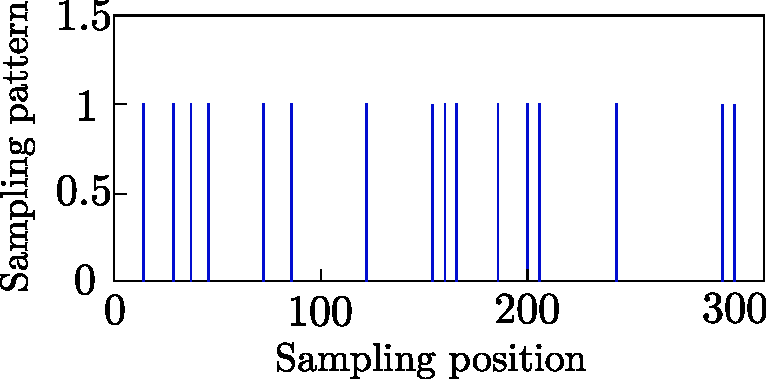
\includegraphics[width=2.6 in]{figs/NUS.pdf}
\DeclareGraphicsExtensions.
\caption{A pseudo-randomly sample pattern for single pure tone signal of length 300}\label{NUS}
\end{figure}

The matrix multiplication between $F$ and $s$ stands for the input signal $x$ which contains sparse spectrum $s$, and $F$ is the full discrete time Fourier transform (DFT) matrix. The diagonal matrix $D$ represents the behavior of non-uniform sampling, where the value $\epsilon$ of diagonal items are chosen pseudo-randomly from $\{0,1\}$. 

The NUS based CS acquisition model establishes a sensing matrix $A$ which equal $DF$ and can be regarded as a random partial Fourier matrix $F_{T}$ which consists of randomly chosen columns of the discrete Fourier matrix (DFT) and indexed by $T$. According to \cite{ragheb2007implementation}, the matrix $A$ satisfies the RIP in compressive sensing so the acquisition model produces a stable reconstruction of $\hat s$ via $l1$-minimisation using $m \geq O(slog(N/s))$ samples\cite{ragheb2007implementation}. In addition, many greedy algorithms such as OMP and CoSaMP are also implemented as fast reconstruction for this architecture \cite{maechler2011random}.

\subsection{Compressive Multiplexer}
\indent \indent Common implementations of the CS based non-uniform sampling architectures varies from \cite{laska2006random, ragheb2007implementation, maechler2011random, rogers2011compressive}. Among these implementations, the random sampling compressive sensing ADC (RS-ADC) is likely to be the prevailing design shown in Figure \ref{RS-ADC}. This architecture is comprised of input multiplexers (MUX), analog queues (AQs), demultiplexer (DEMUX) and a low-rate successive ADC. 
\begin{figure}
\centering
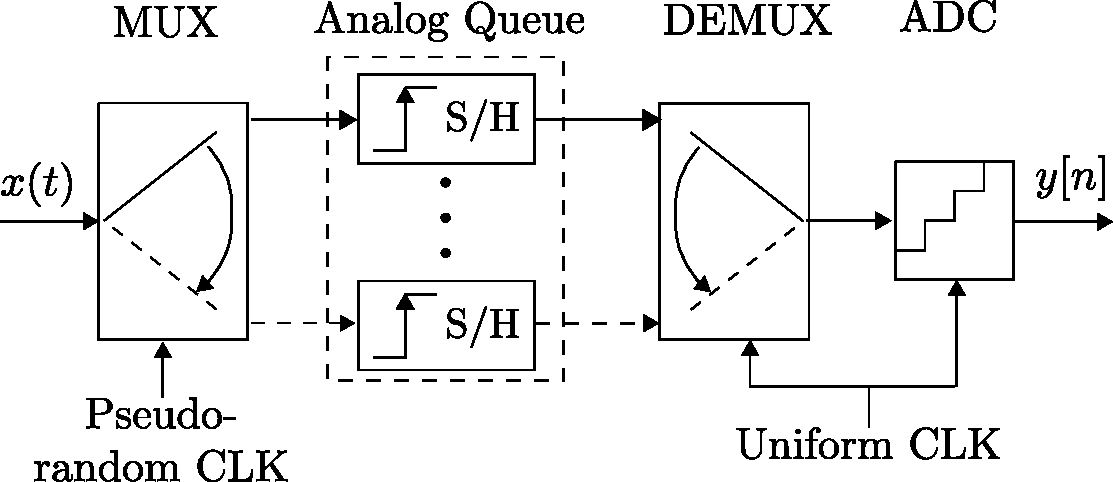
\includegraphics[width=3.0in]{figs/RSADC.pdf}
\DeclareGraphicsExtensions.
\caption{Block diagram of the random sampling CS ADC (RS-ADC). The components includes a pseudo-random sign generator, a low-pass filter, and a sub-Nyquist ADC}\label{RS-ADC}
\end{figure}

This implementation uses an input multiplexer driven by a non-uniform clock to switch the signal among several parallel $S/H$ based analog queues. A low rate ADC (e.g. Successive Approximation ADC) is used to convert the stored samples, performing at uniform intervals but operating at sub-Nyquist average rate. Greedy pursuit algorithms such as OMP and CoSaMP are then used to perform fast reconstruction for this architecture. However, the main problem of applying RS- ADC lies in sampling high frequency signals: since the ADC and input MUX perform inherent bandwidth limitations modeled as a lowpass filter preceding the uniform sampling, acquisitions for high frequency signals results in a loss of the spectrum components. Besides, the high switching speed of the MUX increases noise and reduces the power efficiency.

\section{Conclusion}\label{sct:cs_conclusion}
\indent \indent The Nyquist sampling theorem states that signal should be sampled at least two times faster than the signal bandwidth so that the aliasing would not occur. However, modern applications produce a large amount of data, resulting in large numbers of samples which requires high speed sampling. To overcome this problem, the compressive ADC architectures are studied in this chapter. First we present the theory of CS framework, then a comprehensive survey of the novel compressive ADC (CS-ADC) designs are studied. Major types of CS-ADCs, such as random demodulators, modulated wideband converters, non-uniform samplers, and compressive multiplexer are explained in detail. 

%--------------------------------------------------------------

%\section{Related Works: Sub-Nyquist Analog-to-Digital Convertor}\label{sct:sub-nyquist_adc}
%\indent \indent Compressed Sensing (CS) is a technique XXX
%%cs-rd_intro.tex
\subsection{Wideband Compressed Sensing ADCs}\label{sct:wideband_cs_adc}
Sampling rate is crucial to signal processing systems since high clock rate enhances the power consumption and increases the burden of data transmission and storage. However, it has long been bounded by the Nyquist theory which denotes the minimum sampling rate for traditional acquisition methods, and couldn't reduced easily. In order to overcome this problem, recently many signal processing devices embed CS into analog-to-digital converters (ADCs) and successfully reduces the size of measurements and thus releases the limitation given by the Nyquist theory. As a consequence, the new systems using a relatively lower clock rate significantly outperform the traditional acquisition systems.   

\subsubsection{Random demodulator}
Random demodulator (RD)\cite{tropp2010beyond} is one of the most popular analog-to-digital converters for CS-based signal acquisition and processing. It develops the stability and robustness of CS measurement, and achieves a sub-Nyquist rate ADC for signal sampling and sequentially enhances the system power efficiency.  

\begin{figure}[!b]
\centering
\includegraphics[width=3.2in]{pictures/random_demodulator.pdf}
\DeclareGraphicsExtensions.
\caption{Block diagram of random demodulator (RD). The components includes a pseudo-random sign generator, a low-pass filter, and a sub-Nyquist ADC}\label{RD}
\end{figure}

Figure \ref{RD} shows the construction of the random demodulator: It consists of a pseudo-random sign generator, a low-pass filter, and a sub-Nyquist ADC. The input $K$ sparse signal is first mixed with the chipping sequence $p_c(t)$ which is a waveform and constructed by pseudo-random variables of $\{\pm 1\}$. This chipping sequence is generated by the pseudo-random sign generator which alternates at the Nyquist rate $N$. The mixed production $x(t) \cdot p_c(t)$ then passes through a low pass filter $h(t)$ for anti-aliasing, and finally is sampled by a ADC uniformly at the rate of $m = O(K\log(N/K)) << N$. %N = W , R = M

\subsubsection{Modulated Wideband Convertor}
In the cases of sampling a multi-band signals whose carrier frequencies are unknown or time-variant (blind multi-band signal receiving), the main task is to design a receiver working independently on the carrier frequency at a low rate\cite{mishali2009blind}. Recently, a novel architecture termed modulated wideband converter (MWC) is developed, which applies the CS theory to the traditional blind multi-band signal receivers based on non-uniform sampling\cite{black1980time}. This innovative architecture successfully provides a minimal requirement for the size of observations\cite{mishali2010theory} thus decrease the power consumption.

\begin{figure}[!t]
\centering
\includegraphics[width=3.2in]{pictures/MWC1.pdf}
\DeclareGraphicsExtensions.
\caption{Block diagram of modulated wideband convertor (MWC). The components includes parallel periodic waveforms mixers, low-pass filters, and sub-Nyquist ADCs}\label{MWC1}
\end{figure}

The MWC consists of groups of periodic waveforms, low pass filters and sub-Nyquist rate ADCs, and can be treated as a parallel structure of the random demodulator (RD). As shown in Figure \ref{MWC1}, each group of periodic sequence $p_i(t)$ with minimum interval of $T_p/M$ mixes the input multi-band signal $x(t)$ for shifting the spectrum by $\Delta f_p$ ($f_p = 1/{T_p}$ is the frequency of $p_i(t)$) and filtering it to the baseband for sampling. In the end, low rate ADCs sample the mixed productions at a rate $f_s$ far less than the Nyquist rate $f_{NYQ}$.

Considering the CS measurement MWC, recovering the $\mathbf z(f)$ where each row $X(f-lf_p)$ presents sparse spectrum segments can be regarded as recovering a infinite set of joint sparse vectors. This problem can be solved by changing it to the problem of multiple measurement vectors (MMV)\cite{mishali2008reduce} and has been implemented. 

\subsubsection{CS based signal processing}
Considering that many signal processing applications such as detection, classification, estimation and filtering do not require entire signal reconstruction, and only parts of certain information from measurements are needed, thus we prefer to filter out the useless information before further signal processing. Therefore, if we could estimate the useless information corresponding to some observations $y_I$, and then $throw$ them $away$ before CS based signal recovery, we can avoid a high computational complexity and thus save the power efficiency significantly. This novel idea comes from the compressive signal processing (CSP)\cite{davenport2010signal}.

\subsubsection{Non-Uniform Sampling}
The non-uniform sampling aims at sampling signals in a local Fourier sparse representation\cite{rauhut2010compressive} (LFS) (e.g. wideband signals), and provides an non-uniformly sampling pattern at pseudo-random time points with a low average rate, which establishes a sensing matrix $A$ which can be regarded as a random partial Fourier matrix $F_{T}$ that consists of randomly chosen columns of the discrete Fourier matrix(DFT) and indexed by $T$. According to \cite{ragheb2007implementation}, the matrix $A$ satisfies the RIP in compressive sensing so the acquisition model produces a stable reconstruction of $\hat s$ via $l1$-minimization using $m \geq O(slog(N/s))$ samples\cite{ragheb2007implementation}. 

%\indent \indent 

%--------------------------------------------------------------

%\section{Reconstruction Architecture}\label{sct:imple_fast_recon}

%Impressive progress has been made in fast decades for compressed sensing and its applications. However, the reconstruction for compressive measurements always need long-time execution if accurate and robust results are required, e.g. basis pursuit requires $O(N^3)$ running time which far larger than $O(kmn)$ in algorithms like orthogonal matching pursuit in \ref{omp}. 

%In other words, computational efforts for high performance recovery of compressive measurements are still difficult and crucial. In this section, some general matching pursuit based recovery architectures are introduced, and the motivation of compressive signal processing (CSP) is mentioned.

%However, the computational effort for successful signal recovery remains high, even for problems of moderate size. Reconstruction becomes especially challenging for real-time applications with stringent power constraints, e.g., on mobile devices. Such applications require efficient hardware implementations of sparse signal recovery algorithms, which we develop in this thesis. We present different architectures of greedy algorithms for a number of selected applications. The first example is the estimation of sparse channels in broad-band wireless communication. The use of sparse recovery algorithms efficiently reduces noise and, thus, increases estimation quality. Architectures for three algorithms are developed and their realisations. in application-specific integrated circuits (ASICs) are compared. We show that approximative algorithms deliver good results at low hard- ware complexity. The second application is the recovery of signals corrupted by structured noise. Using the example of audio restoration from corruptions by clicks and pops, fast realisations of the approximate message passing algorithm are designed. Two fundamentally different architectures —one relying on fast transforms, the other relying on parallel processing power—are developed and compared. Large gains in terms of throughput and circuit complexity are realised by applying fast transforms in the context of CS recovery. The choice of the most attractive algorithms and architectures depends on the sparsity, the number of measurements, and the basis in which the samples are taken. In general, approximate message passing is found to be very well suited for hardware recovery of moderately sparse signals while serial greedy pursuits are better suited for very sparse signals.
%} 

%------------
% parallel ..
% hardware OMP. 
% AMP ..
% CoSaMP
%------------

%re-wr{
%The introduction of compressive sensing (CS) led to a new paradigm in signal processing. Traditionally, signals are sampled above their Nyquist rate. Using CS, the same information is acquired with much fewer measurements, provided a sparse representation of the signal exists. This makes CS a very promising technology with a large number of potential applications.
%While the acquisition of measurements is simplified, the reconstruction of the original signal becomes more involved. Sparse signal recovery algorithms solve the corresponding systems of underdetermined linear equations and have proven very efficient for various applications. 
%Examples include de-noising, the restoration of corrupted signals, signal separation, super-resolution, and in-painting. All applications are based on the observation that many natural and man-made signals have sparse representations in some suitable bases.
%}
%In this chapter, we give a review of the theory of compressed sensing system. In addition, the typical applications in radar system and medical scanners (e.g. magnetic resonance imaging, MRI) are introduced. Moreover, we focus on our related work for a survey of potential analog-to-digital convertors for future wireless devices.
%------


%----description of CS-MUX ----
%The workflow of RS-ADC can be described as the following steps: At first, it orderly dispatched the input analog signal through a multiplexer which is driven by a non-uniform clock. Then, the system store the dispatched analog signal in different analog queues using sample and hold (S/H). At last, the demultiplexer driven by a periodic clock sequentially selects the output of the analog queue and transfers the value to the low-rate ADC. Considering the modulated based CS-ADC such as the RD and MWC, the NUS such as RS-ADC is an alternative architecture to establish a constructed pseudo-random measurement for CS based ADC design. Compared to the RD and MWC, the advantage of RS-ADC stays in the fact that it saves power consumption and chip area since it doesn’t need to mix a high rate chipping sequence and only contains a single ADC. However, the main drawback of the NUS is obvious non-idealism caused by the timing jitter. The timing jitter, which derives from the input multiplexer, brings sample error and propagates it through the entire system thus produces additional noise and critical inaccuracy. Moreover, switch capacitors and delay in multiplexers also reduces the robustness of the RS-ADC systems. 


% ---- desciption of RD -----
%It consists of a pseudo-random sign generator, a low-pass filter, and a sub-Nyquist ADC. The input $K$ sparse signal is first mixed with the chipping sequence $p_c(t)$ which is a waveform and constructed by pseudo-random variables of $\{\pm 1\}$. This chipping sequence is generated by the pseudo-random sign generator which alternates at the Nyquist rate $N$. The mixed production $x(t) \cdot p_c(t)$ then passes through a low pass filter $h(t)$ for anti-aliasing, and finally is sampled by a ADC uniformly at the rate of $m = O(K\log(N/K)) << N$. This design is simple, but easily affected by model mismatches and design imperfections.
